% Editable native annotations around unchanged, verified IDE photographs.
\par
\begin{figure}[htbp]
\centering
\sbox0{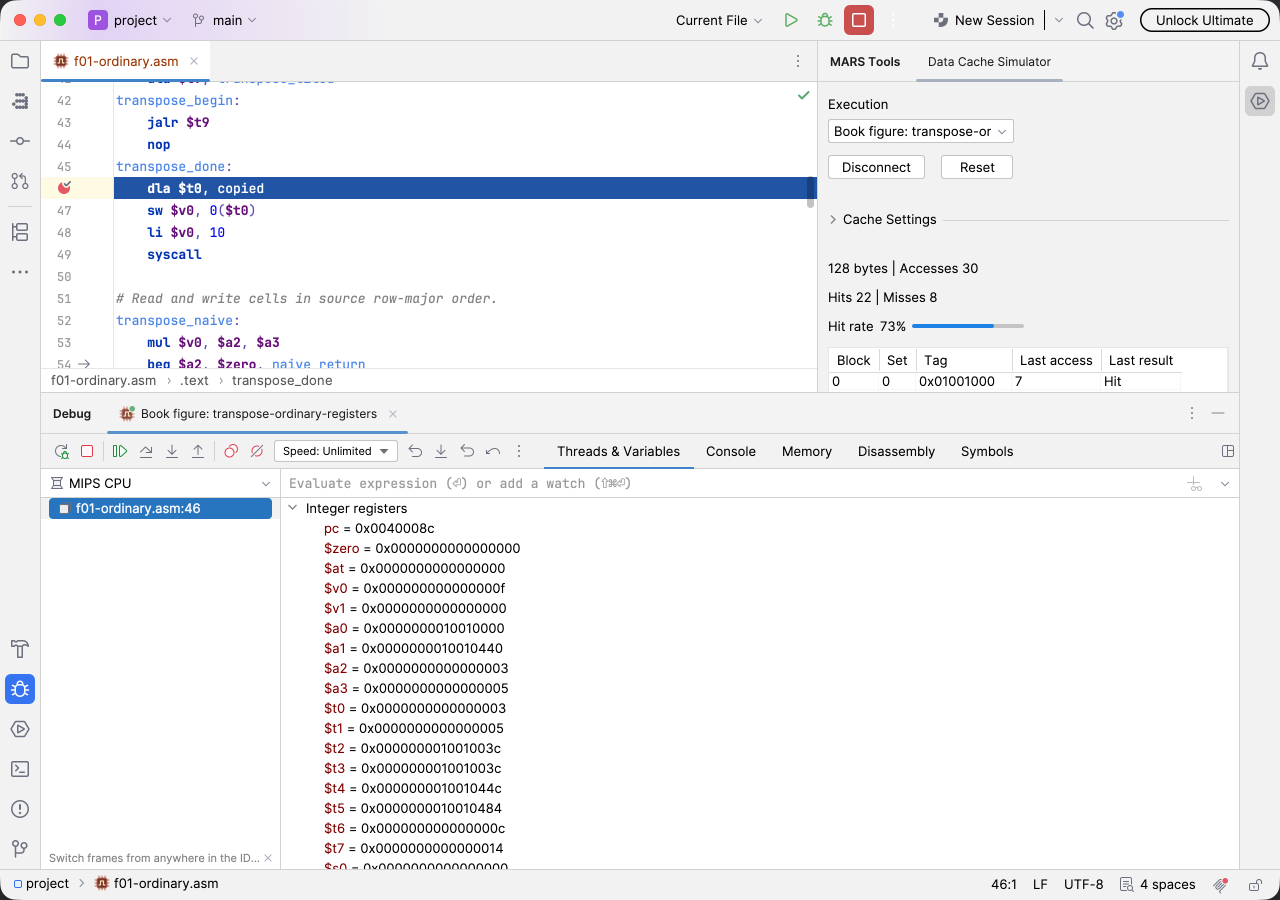
\includegraphics[artifact]{packages/011-matrix-transpose/captures/f01-ordinary/registers.png}}
\sbox2{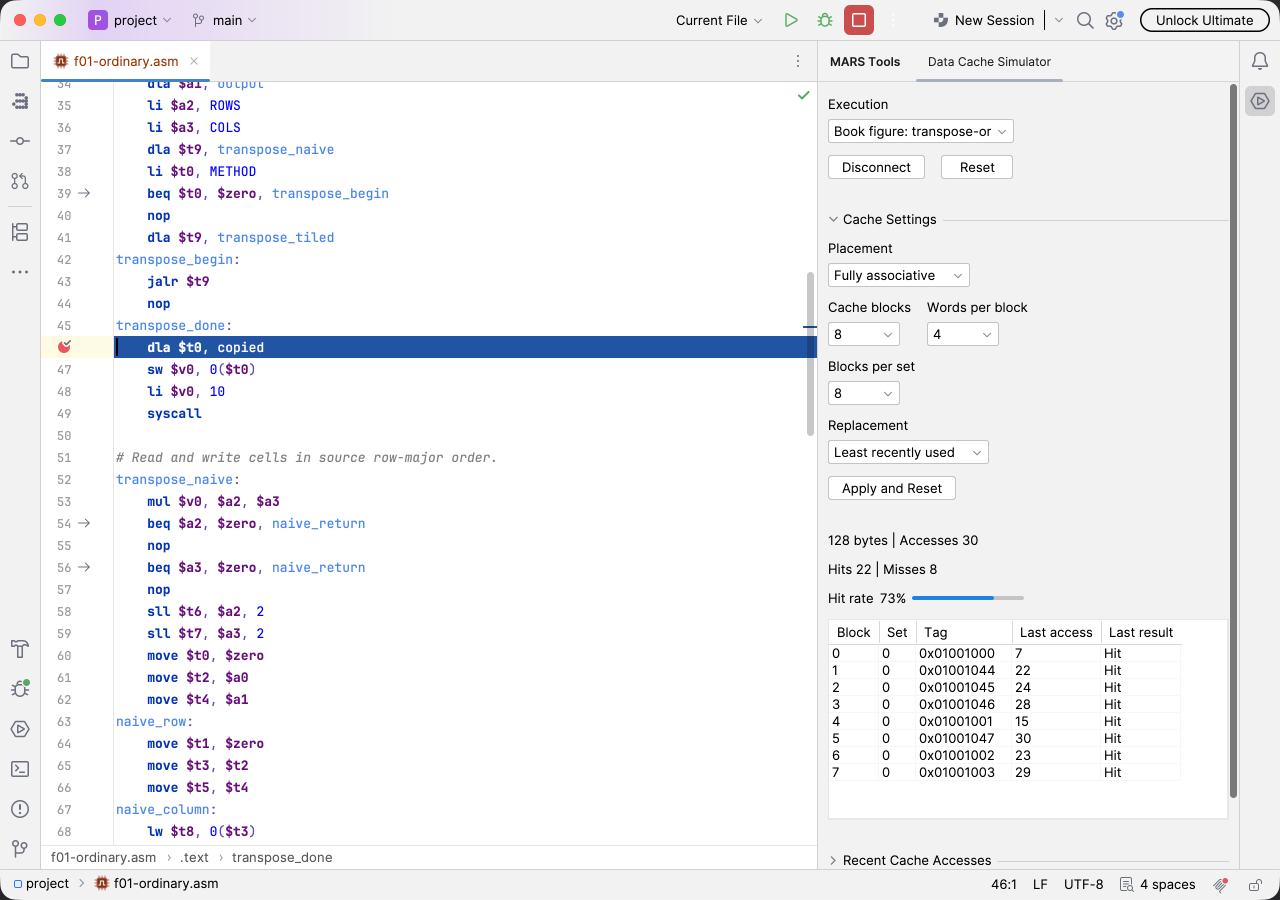
\includegraphics[artifact]{packages/011-matrix-transpose/captures/f01-ordinary/cache.png}}
\sbox4{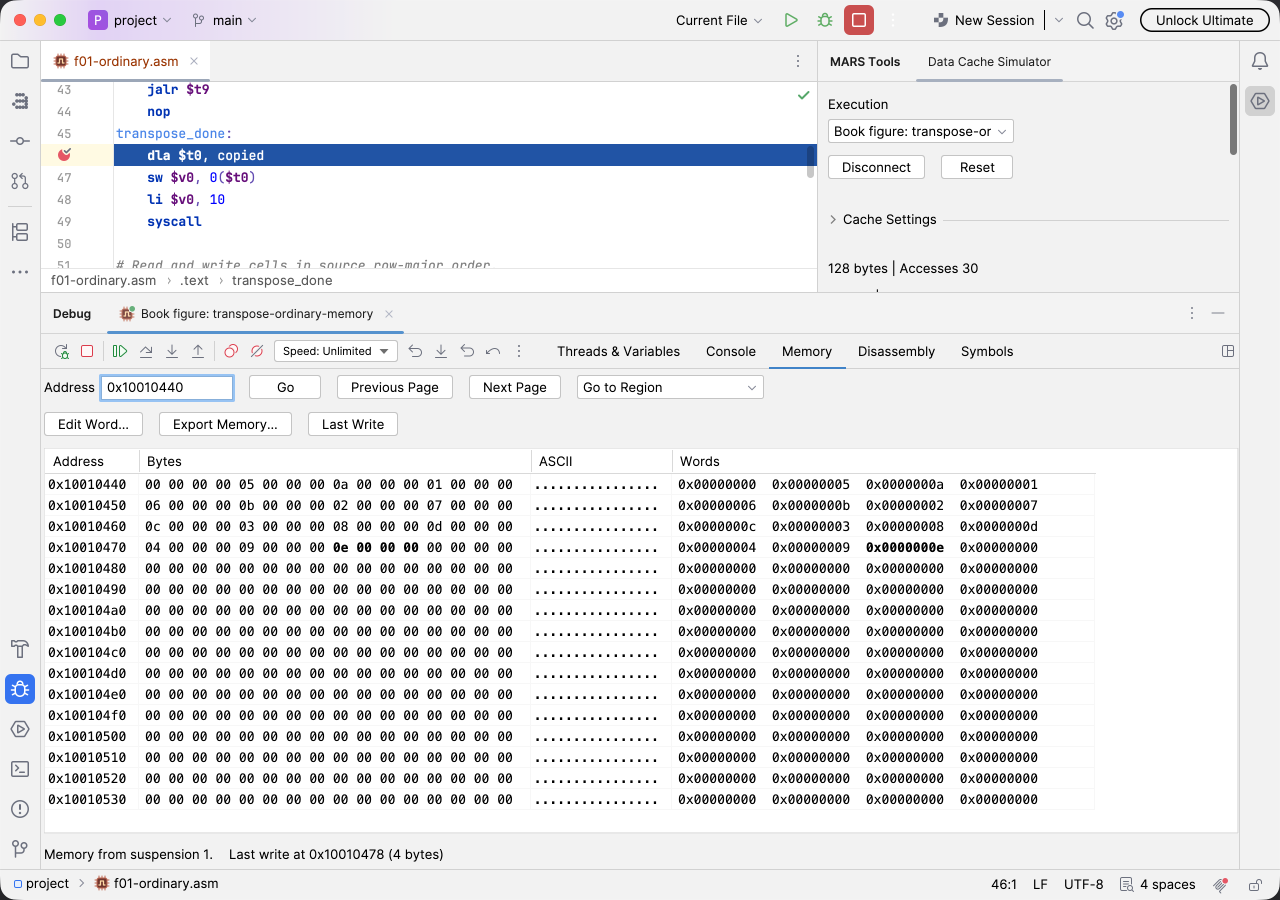
\includegraphics[artifact]{packages/011-matrix-transpose/captures/f01-ordinary/memory.png}}
\edef\MARStransposeordinarysourceLeft{\the\dimexpr0.036718750\wd0\relax}
\edef\MARStransposeordinarysourceBottom{\the\dimexpr0.774444444\ht0\relax}
\edef\MARStransposeordinarysourceRight{\the\dimexpr0.713281250\wd0\relax}
\edef\MARStransposeordinarysourceTop{\the\dimexpr0.147777778\ht0\relax}
\edef\MARStransposeordinaryregistersLeft{\the\dimexpr0.246093750\wd0\relax}
\edef\MARStransposeordinaryregistersBottom{\the\dimexpr0.220000000\ht0\relax}
\edef\MARStransposeordinaryregistersRight{\the\dimexpr0.596875000\wd0\relax}
\edef\MARStransposeordinaryregistersTop{\the\dimexpr0.637777778\ht0\relax}
\edef\MARStransposeordinarygeometryLeft{\the\dimexpr0.639843750\wd2\relax}
\edef\MARStransposeordinarygeometryBottom{\the\dimexpr0.476666667\ht2\relax}
\edef\MARStransposeordinarygeometryRight{\the\dimexpr0.192187500\wd2\relax}
\edef\MARStransposeordinarygeometryTop{\the\dimexpr0.262222222\ht2\relax}
\edef\MARStransposeordinarycountersLeft{\the\dimexpr0.642187500\wd2\relax}
\edef\MARStransposeordinarycountersBottom{\the\dimexpr0.321111111\ht2\relax}
\edef\MARStransposeordinarycountersRight{\the\dimexpr0.035156250\wd2\relax}
\edef\MARStransposeordinarycountersTop{\the\dimexpr0.586666667\ht2\relax}
\edef\MARStransposeordinarymemoryLeft{\the\dimexpr0.034375000\wd4\relax}
\edef\MARStransposeordinarymemoryBottom{\the\dimexpr0.375555556\ht4\relax}
\edef\MARStransposeordinarymemoryRight{\the\dimexpr0.584375000\wd4\relax}
\edef\MARStransposeordinarymemoryTop{\the\dimexpr0.497777778\ht4\relax}
\begin{tikzpicture}[alt={Five annotated details from the same ordinary transpose boundary. Rows is three, columns five and the returned count fifteen. Output contains five rows of three words. The 128-byte fully associative cache records thirty accesses, twenty-two hits and eight misses, or a rounded seventy-three percent hit rate.}]
\node[anchor=north west,inner sep=0,font=\small\bfseries] (source-title) at (6mm,0) {Next instruction};
\node[anchor=north west,inner sep=0] (source) at ([yshift=-1mm]source-title.south west) {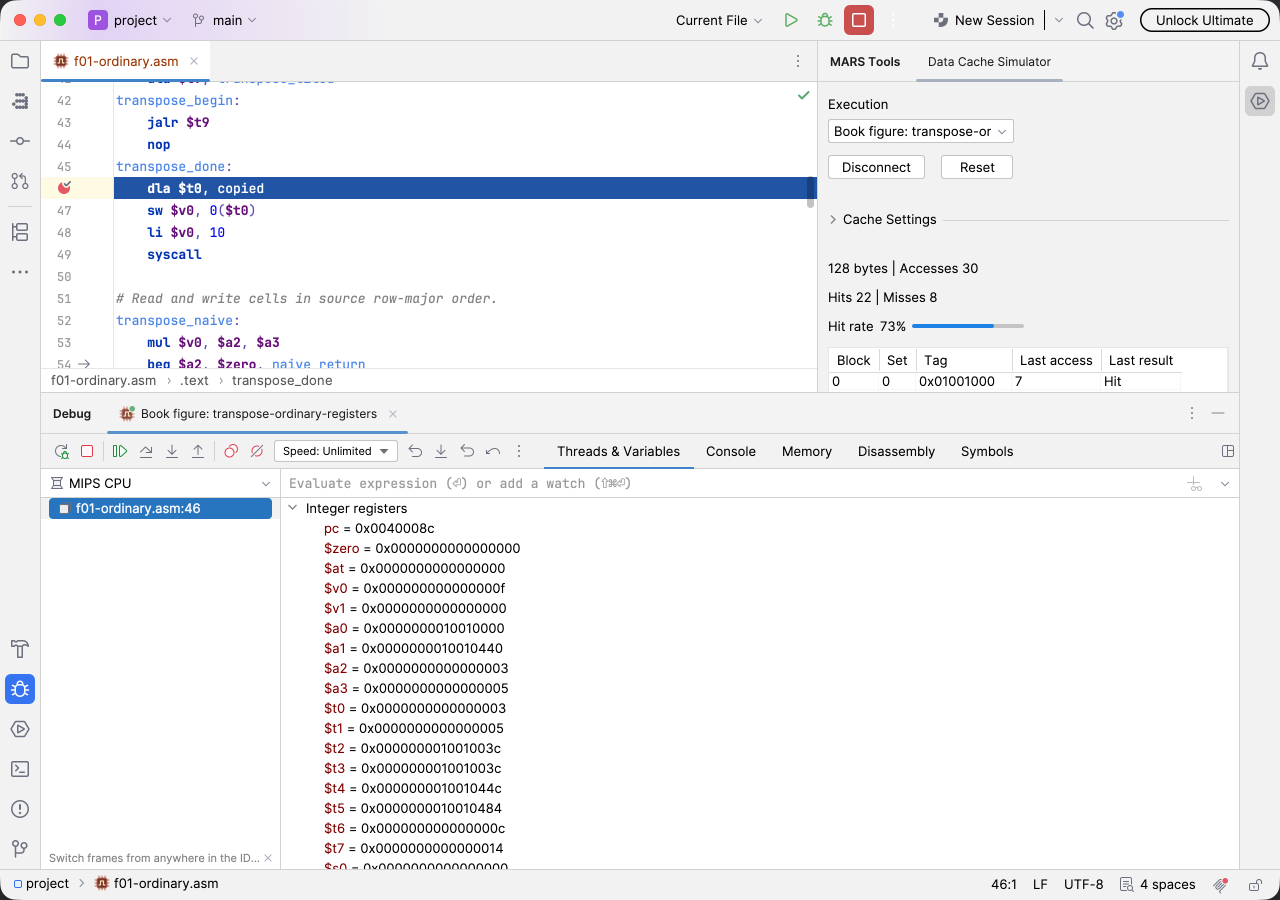
\includegraphics[width=0.5\linewidth,artifact,trim={\MARStransposeordinarysourceLeft{} \MARStransposeordinarysourceBottom{} \MARStransposeordinarysourceRight{} \MARStransposeordinarysourceTop{}},clip]{packages/011-matrix-transpose/captures/f01-ordinary/registers.png}};
\begin{scope}[shift={(source.south west)},x={($(source.south east)-(source.south west)$)},y={($(source.north west)-(source.south west)$)}]
\draw[black,line width=0.7pt] (0.215625000,0.057142857) rectangle (0.678125000,0.371428571);
\node[draw=black,fill=white,circle,inner sep=1.5pt,font=\footnotesize] at ($(0.215625000,0.371428571)+(-3mm,0)$) {1};
\end{scope}
\node[anchor=north west,inner sep=0,font=\small\bfseries] (registers-title) at ([yshift=-2mm]source.south west) {Dimensions and count};
\node[anchor=north west,inner sep=0] (registers) at ([yshift=-1mm]registers-title.south west) {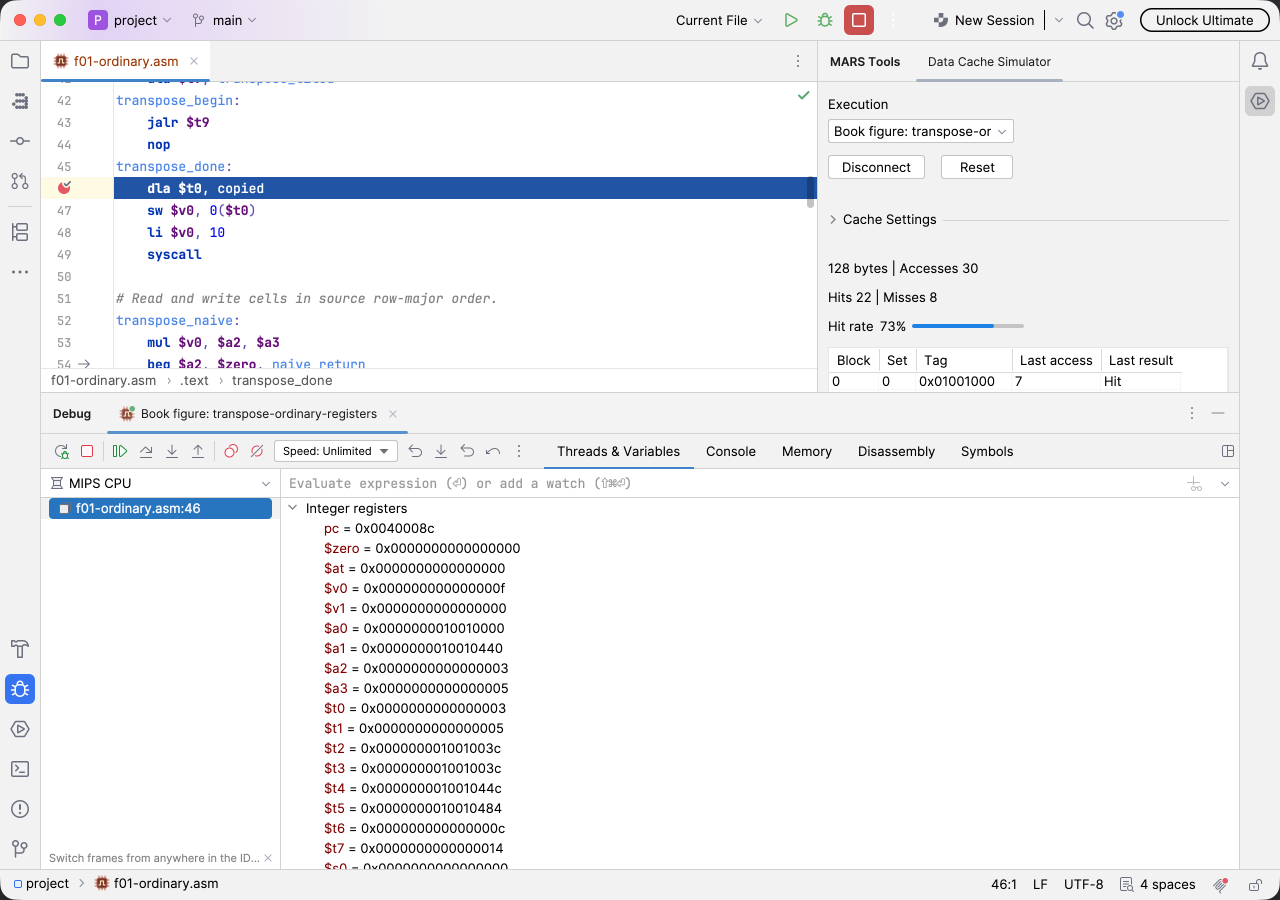
\includegraphics[width=0.33\linewidth,artifact,trim={\MARStransposeordinaryregistersLeft{} \MARStransposeordinaryregistersBottom{} \MARStransposeordinaryregistersRight{} \MARStransposeordinaryregistersTop{}},clip]{packages/011-matrix-transpose/captures/f01-ordinary/registers.png}};
\begin{scope}[shift={(registers.south west)},x={($(registers.south east)-(registers.south west)$)},y={($(registers.north west)-(registers.south west)$)}]
\draw[black,line width=0.7pt] (0.029850746,0.031250000) rectangle (0.970149254,0.968750000);
\node[draw=black,fill=white,circle,inner sep=1.5pt,font=\footnotesize] at ($(0.029850746,0.968750000)+(-3mm,0)$) {2};
\end{scope}
\node[anchor=north west,inner sep=0,font=\small\bfseries] (geometry-title) at (0.60\linewidth,0) {Cache geometry and policy};
\node[anchor=north west,inner sep=0] (geometry) at ([yshift=-1mm]geometry-title.south west) {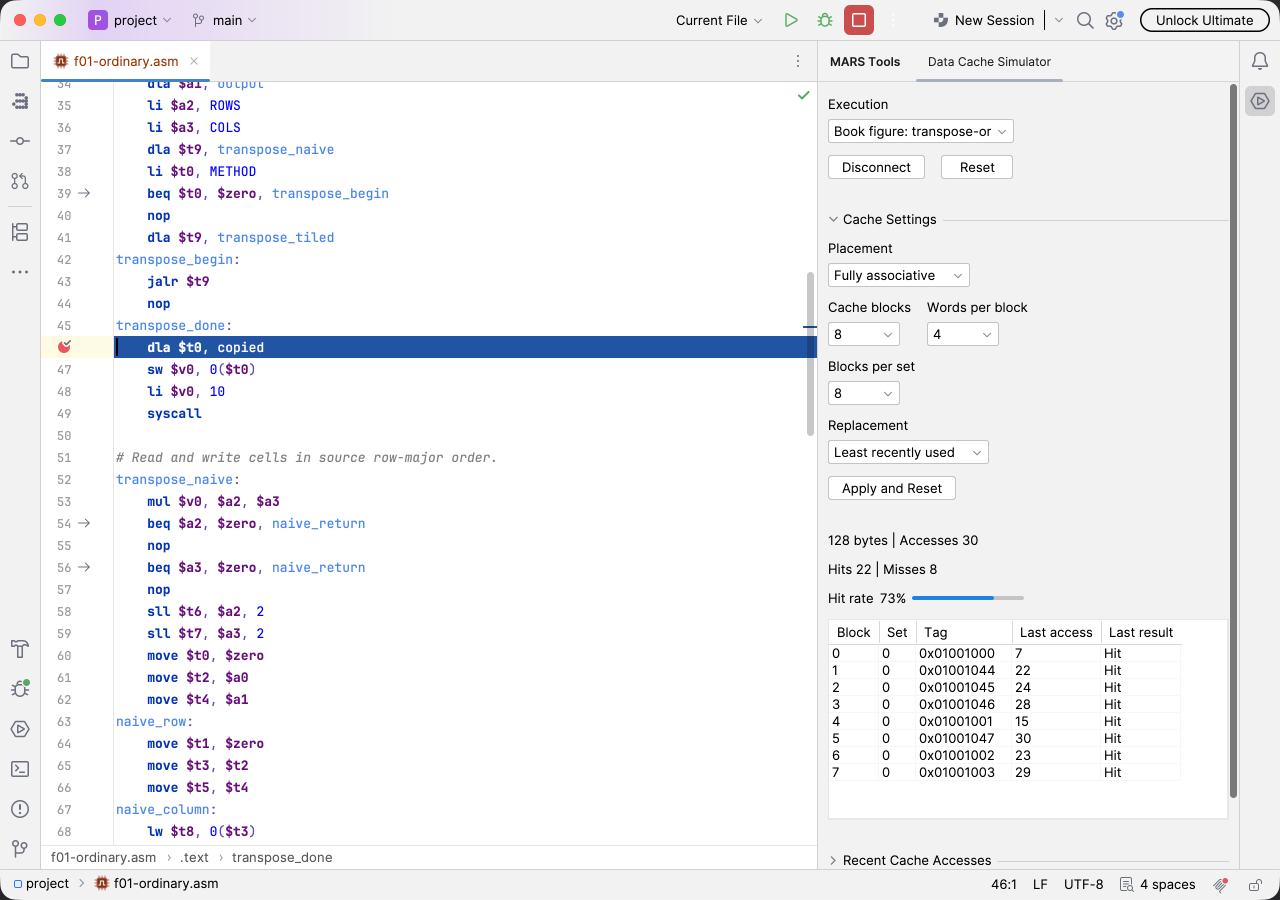
\includegraphics[width=0.31\linewidth,artifact,trim={\MARStransposeordinarygeometryLeft{} \MARStransposeordinarygeometryBottom{} \MARStransposeordinarygeometryRight{} \MARStransposeordinarygeometryTop{}},clip]{packages/011-matrix-transpose/captures/f01-ordinary/cache.png}};
\begin{scope}[shift={(geometry.south west)},x={($(geometry.south east)-(geometry.south west)$)},y={($(geometry.north west)-(geometry.south west)$)}]
\draw[black,line width=0.7pt] (0.027906977,0.017021277) rectangle (0.972093023,0.982978723);
\node[draw=black,fill=white,circle,inner sep=1.5pt,font=\footnotesize] at ($(0.027906977,0.982978723)+(-3mm,0)$) {3};
\end{scope}
\node[anchor=north west,inner sep=0,font=\small\bfseries] (counters-title) at ([yshift=-8mm]6mm,0 |- geometry.south) {Data-access counters};
\node[anchor=north west,inner sep=0] (counters) at ([yshift=-1mm]counters-title.south west) {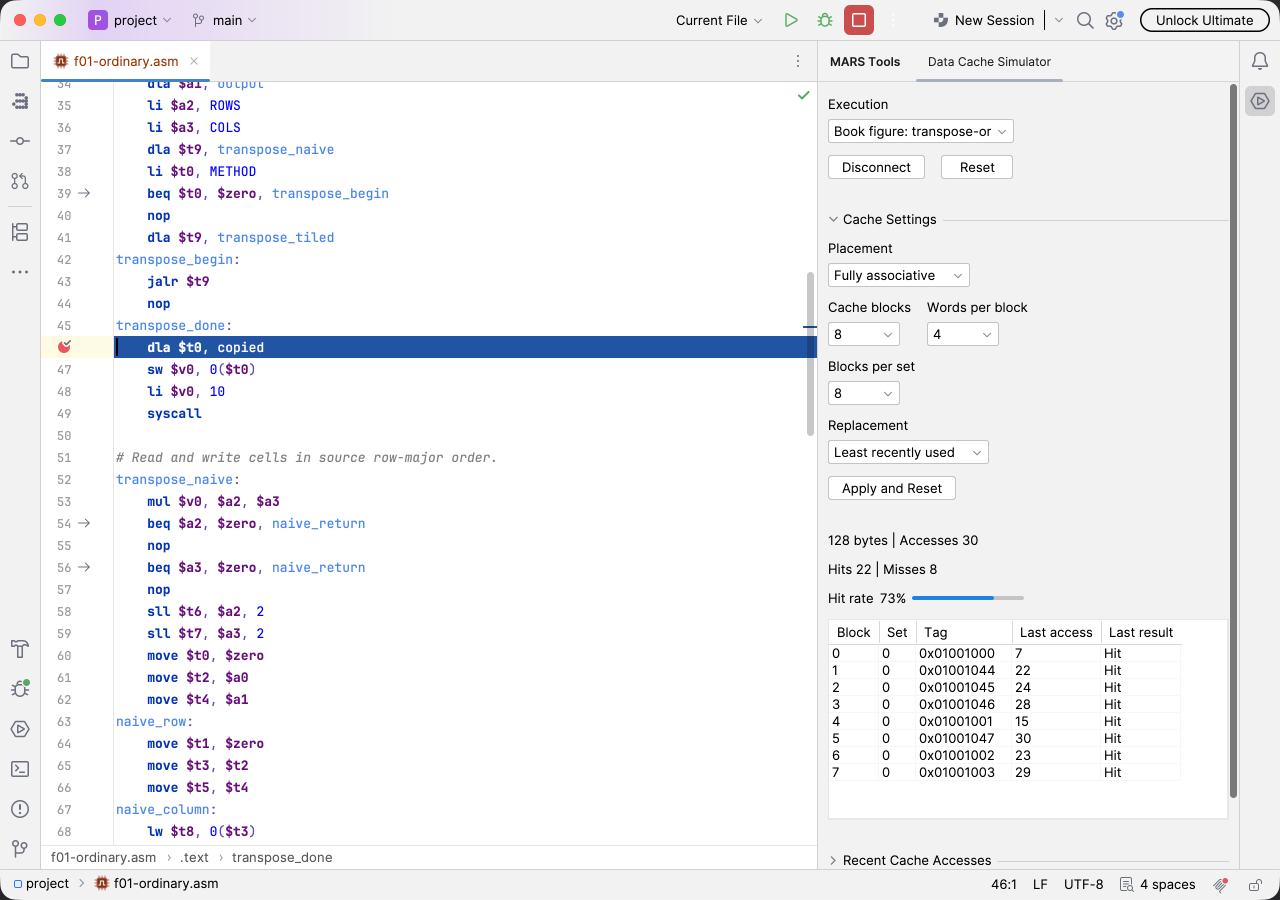
\includegraphics[width=0.60\linewidth,artifact,trim={\MARStransposeordinarycountersLeft{} \MARStransposeordinarycountersBottom{} \MARStransposeordinarycountersRight{} \MARStransposeordinarycountersTop{}},clip]{packages/011-matrix-transpose/captures/f01-ordinary/cache.png}};
\begin{scope}[shift={(counters.south west)},x={($(counters.south east)-(counters.south west)$)},y={($(counters.north west)-(counters.south west)$)}]
\draw[black,line width=0.7pt] (0.014527845,0.048192771) rectangle (0.985472155,0.951807229);
\node[draw=black,fill=white,circle,inner sep=1.5pt,font=\footnotesize] at ($(0.014527845,0.951807229)+(-3mm,0)$) {4};
\end{scope}
\node[anchor=north west,inner sep=0,font=\small\bfseries] (memory-title) at ([yshift=-4mm]6mm,0 |- counters.south) {Output addresses and little-endian bytes};
\node[anchor=north west,inner sep=0] (memory) at ([yshift=-1mm]memory-title.south west) {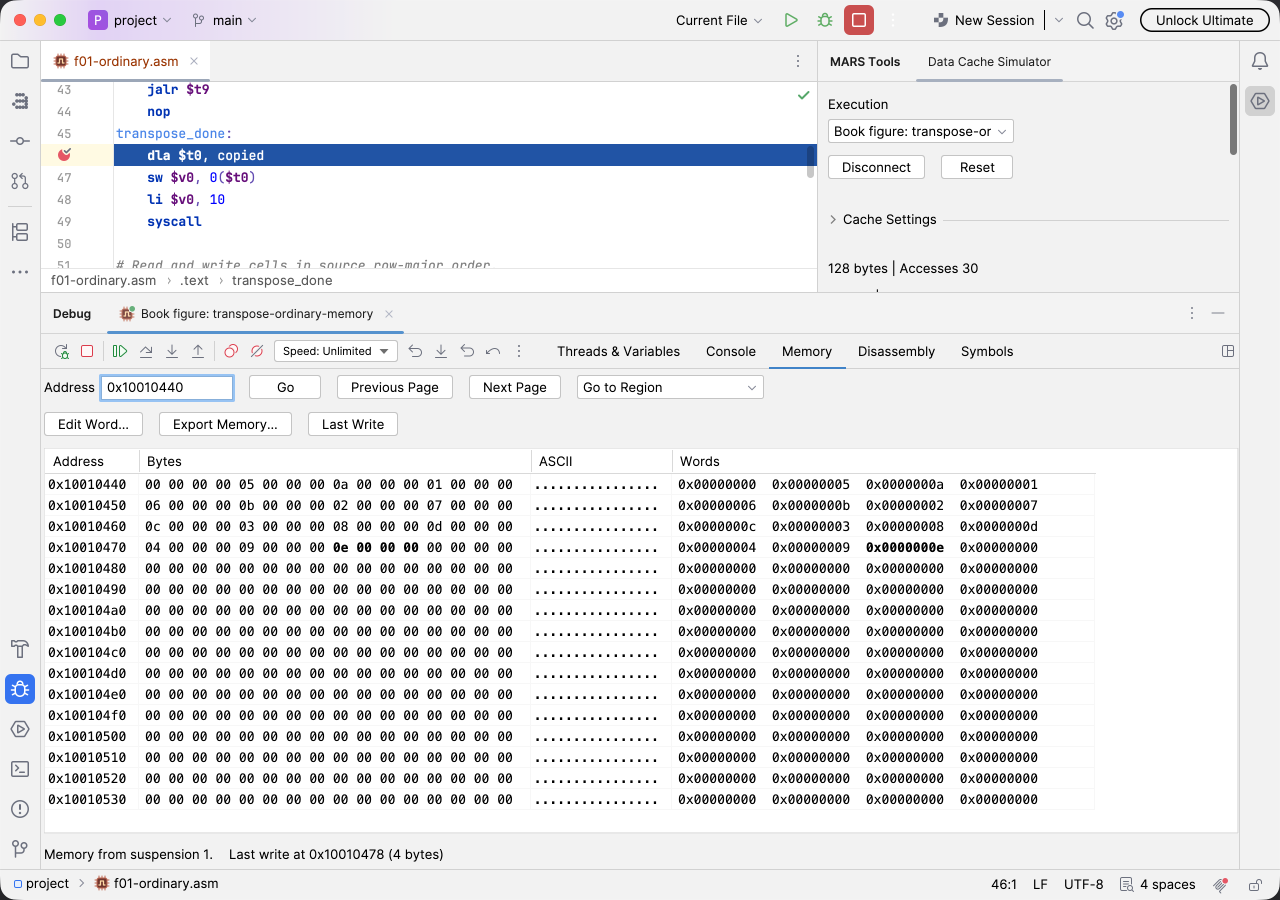
\includegraphics[width=0.78\linewidth,artifact,trim={\MARStransposeordinarymemoryLeft{} \MARStransposeordinarymemoryBottom{} \MARStransposeordinarymemoryRight{} \MARStransposeordinarymemoryTop{}},clip]{packages/011-matrix-transpose/captures/f01-ordinary/memory.png}};
\begin{scope}[shift={(memory.south west)},x={($(memory.south east)-(memory.south west)$)},y={($(memory.north west)-(memory.south west)$)}]
\draw[black,line width=0.7pt] (0.194672131,0.035087719) rectangle (0.997950820,0.771929825);
\node[draw=black,fill=white,circle,inner sep=1.5pt,font=\footnotesize] at ($(0.194672131,0.771929825)+(-3mm,0)$) {5};
\end{scope}
\end{tikzpicture}
\par\smallskip
\begin{minipage}{\linewidth}
\small
\begin{enumerate}
\setlength{\itemsep}{2pt}
\setlength{\parsep}{0pt}
\item The blue \texttt{dla \$t0, copied} is next at \texttt{transpose\_done}. The routine has returned; the caller has not stored its result. The following \texttt{sw} would add one data access.
\item The input dimensions remain \texttt{\$a2 = 3} and \texttt{\$a3 = 5}. The returned \texttt{\$v0 = 0x0f} is decimal 15. Transposition gives five output rows of three, with the same element count.
\item Eight blocks, four words per block and four bytes per word give $8\times4\times4=128$ bytes. Eight blocks per set makes one fully associative set; replacement is least recently used.
\item Thirty accesses are fifteen loads plus fifteen stores. Eight misses leave 22 hits, giving $22/30\approx73\%$. The model observes data accesses only; this percentage is not an elapsed-time or processor-cycle measurement.
\item At \texttt{0x10010440}, read four little-endian bytes per word. The first words are $0,5,10,1$; \texttt{0a 00 00 00} represents decimal 10. The fifteen active words form rows $[0,5,10]$, $[1,6,11]$, $[2,7,12]$, $[3,8,13]$ and $[4,9,14]$. Each debugger line groups four words, so a displayed line is not a matrix row. The sixteenth word is outside the active output.
\end{enumerate}
\end{minipage}
\caption{The ordinary transpose returns fifteen elements before the caller stores the count.}
\label{capture:011-matrix-transpose-f01-ordinary}
\label{transpose-f01-ordinary}
\end{figure}
\par
